% Options for packages loaded elsewhere
\PassOptionsToPackage{unicode}{hyperref}
\PassOptionsToPackage{hyphens}{url}
%
\documentclass[
]{article}
\usepackage{lmodern}
\usepackage{amssymb,amsmath}
\usepackage{ifxetex,ifluatex}
\ifnum 0\ifxetex 1\fi\ifluatex 1\fi=0 % if pdftex
  \usepackage[T1]{fontenc}
  \usepackage[utf8]{inputenc}
  \usepackage{textcomp} % provide euro and other symbols
\else % if luatex or xetex
  \usepackage{unicode-math}
  \defaultfontfeatures{Scale=MatchLowercase}
  \defaultfontfeatures[\rmfamily]{Ligatures=TeX,Scale=1}
\fi
% Use upquote if available, for straight quotes in verbatim environments
\IfFileExists{upquote.sty}{\usepackage{upquote}}{}
\IfFileExists{microtype.sty}{% use microtype if available
  \usepackage[]{microtype}
  \UseMicrotypeSet[protrusion]{basicmath} % disable protrusion for tt fonts
}{}
\makeatletter
\@ifundefined{KOMAClassName}{% if non-KOMA class
  \IfFileExists{parskip.sty}{%
    \usepackage{parskip}
  }{% else
    \setlength{\parindent}{0pt}
    \setlength{\parskip}{6pt plus 2pt minus 1pt}}
}{% if KOMA class
  \KOMAoptions{parskip=half}}
\makeatother
\usepackage{xcolor}
\IfFileExists{xurl.sty}{\usepackage{xurl}}{} % add URL line breaks if available
\IfFileExists{bookmark.sty}{\usepackage{bookmark}}{\usepackage{hyperref}}
\hypersetup{
  pdftitle={Data 605 HW 13},
  pdfauthor={Gabe Abreu},
  hidelinks,
  pdfcreator={LaTeX via pandoc}}
\urlstyle{same} % disable monospaced font for URLs
\usepackage[margin=1in]{geometry}
\usepackage{color}
\usepackage{fancyvrb}
\newcommand{\VerbBar}{|}
\newcommand{\VERB}{\Verb[commandchars=\\\{\}]}
\DefineVerbatimEnvironment{Highlighting}{Verbatim}{commandchars=\\\{\}}
% Add ',fontsize=\small' for more characters per line
\usepackage{framed}
\definecolor{shadecolor}{RGB}{248,248,248}
\newenvironment{Shaded}{\begin{snugshade}}{\end{snugshade}}
\newcommand{\AlertTok}[1]{\textcolor[rgb]{0.94,0.16,0.16}{#1}}
\newcommand{\AnnotationTok}[1]{\textcolor[rgb]{0.56,0.35,0.01}{\textbf{\textit{#1}}}}
\newcommand{\AttributeTok}[1]{\textcolor[rgb]{0.77,0.63,0.00}{#1}}
\newcommand{\BaseNTok}[1]{\textcolor[rgb]{0.00,0.00,0.81}{#1}}
\newcommand{\BuiltInTok}[1]{#1}
\newcommand{\CharTok}[1]{\textcolor[rgb]{0.31,0.60,0.02}{#1}}
\newcommand{\CommentTok}[1]{\textcolor[rgb]{0.56,0.35,0.01}{\textit{#1}}}
\newcommand{\CommentVarTok}[1]{\textcolor[rgb]{0.56,0.35,0.01}{\textbf{\textit{#1}}}}
\newcommand{\ConstantTok}[1]{\textcolor[rgb]{0.00,0.00,0.00}{#1}}
\newcommand{\ControlFlowTok}[1]{\textcolor[rgb]{0.13,0.29,0.53}{\textbf{#1}}}
\newcommand{\DataTypeTok}[1]{\textcolor[rgb]{0.13,0.29,0.53}{#1}}
\newcommand{\DecValTok}[1]{\textcolor[rgb]{0.00,0.00,0.81}{#1}}
\newcommand{\DocumentationTok}[1]{\textcolor[rgb]{0.56,0.35,0.01}{\textbf{\textit{#1}}}}
\newcommand{\ErrorTok}[1]{\textcolor[rgb]{0.64,0.00,0.00}{\textbf{#1}}}
\newcommand{\ExtensionTok}[1]{#1}
\newcommand{\FloatTok}[1]{\textcolor[rgb]{0.00,0.00,0.81}{#1}}
\newcommand{\FunctionTok}[1]{\textcolor[rgb]{0.00,0.00,0.00}{#1}}
\newcommand{\ImportTok}[1]{#1}
\newcommand{\InformationTok}[1]{\textcolor[rgb]{0.56,0.35,0.01}{\textbf{\textit{#1}}}}
\newcommand{\KeywordTok}[1]{\textcolor[rgb]{0.13,0.29,0.53}{\textbf{#1}}}
\newcommand{\NormalTok}[1]{#1}
\newcommand{\OperatorTok}[1]{\textcolor[rgb]{0.81,0.36,0.00}{\textbf{#1}}}
\newcommand{\OtherTok}[1]{\textcolor[rgb]{0.56,0.35,0.01}{#1}}
\newcommand{\PreprocessorTok}[1]{\textcolor[rgb]{0.56,0.35,0.01}{\textit{#1}}}
\newcommand{\RegionMarkerTok}[1]{#1}
\newcommand{\SpecialCharTok}[1]{\textcolor[rgb]{0.00,0.00,0.00}{#1}}
\newcommand{\SpecialStringTok}[1]{\textcolor[rgb]{0.31,0.60,0.02}{#1}}
\newcommand{\StringTok}[1]{\textcolor[rgb]{0.31,0.60,0.02}{#1}}
\newcommand{\VariableTok}[1]{\textcolor[rgb]{0.00,0.00,0.00}{#1}}
\newcommand{\VerbatimStringTok}[1]{\textcolor[rgb]{0.31,0.60,0.02}{#1}}
\newcommand{\WarningTok}[1]{\textcolor[rgb]{0.56,0.35,0.01}{\textbf{\textit{#1}}}}
\usepackage{graphicx,grffile}
\makeatletter
\def\maxwidth{\ifdim\Gin@nat@width>\linewidth\linewidth\else\Gin@nat@width\fi}
\def\maxheight{\ifdim\Gin@nat@height>\textheight\textheight\else\Gin@nat@height\fi}
\makeatother
% Scale images if necessary, so that they will not overflow the page
% margins by default, and it is still possible to overwrite the defaults
% using explicit options in \includegraphics[width, height, ...]{}
\setkeys{Gin}{width=\maxwidth,height=\maxheight,keepaspectratio}
% Set default figure placement to htbp
\makeatletter
\def\fps@figure{htbp}
\makeatother
\setlength{\emergencystretch}{3em} % prevent overfull lines
\providecommand{\tightlist}{%
  \setlength{\itemsep}{0pt}\setlength{\parskip}{0pt}}
\setcounter{secnumdepth}{-\maxdimen} % remove section numbering

\title{Data 605 HW 13}
\author{Gabe Abreu}
\date{11/29/2020}

\begin{document}
\maketitle

\hypertarget{assignment-13}{%
\subsection{Assignment 13}\label{assignment-13}}

1.Use integration by substitution to solve the integral below

\begin{Shaded}
\begin{Highlighting}[]
\NormalTok{knitr}\OperatorTok{::}\KeywordTok{include_graphics}\NormalTok{(}\StringTok{'13_1.jpg'}\NormalTok{)}
\end{Highlighting}
\end{Shaded}

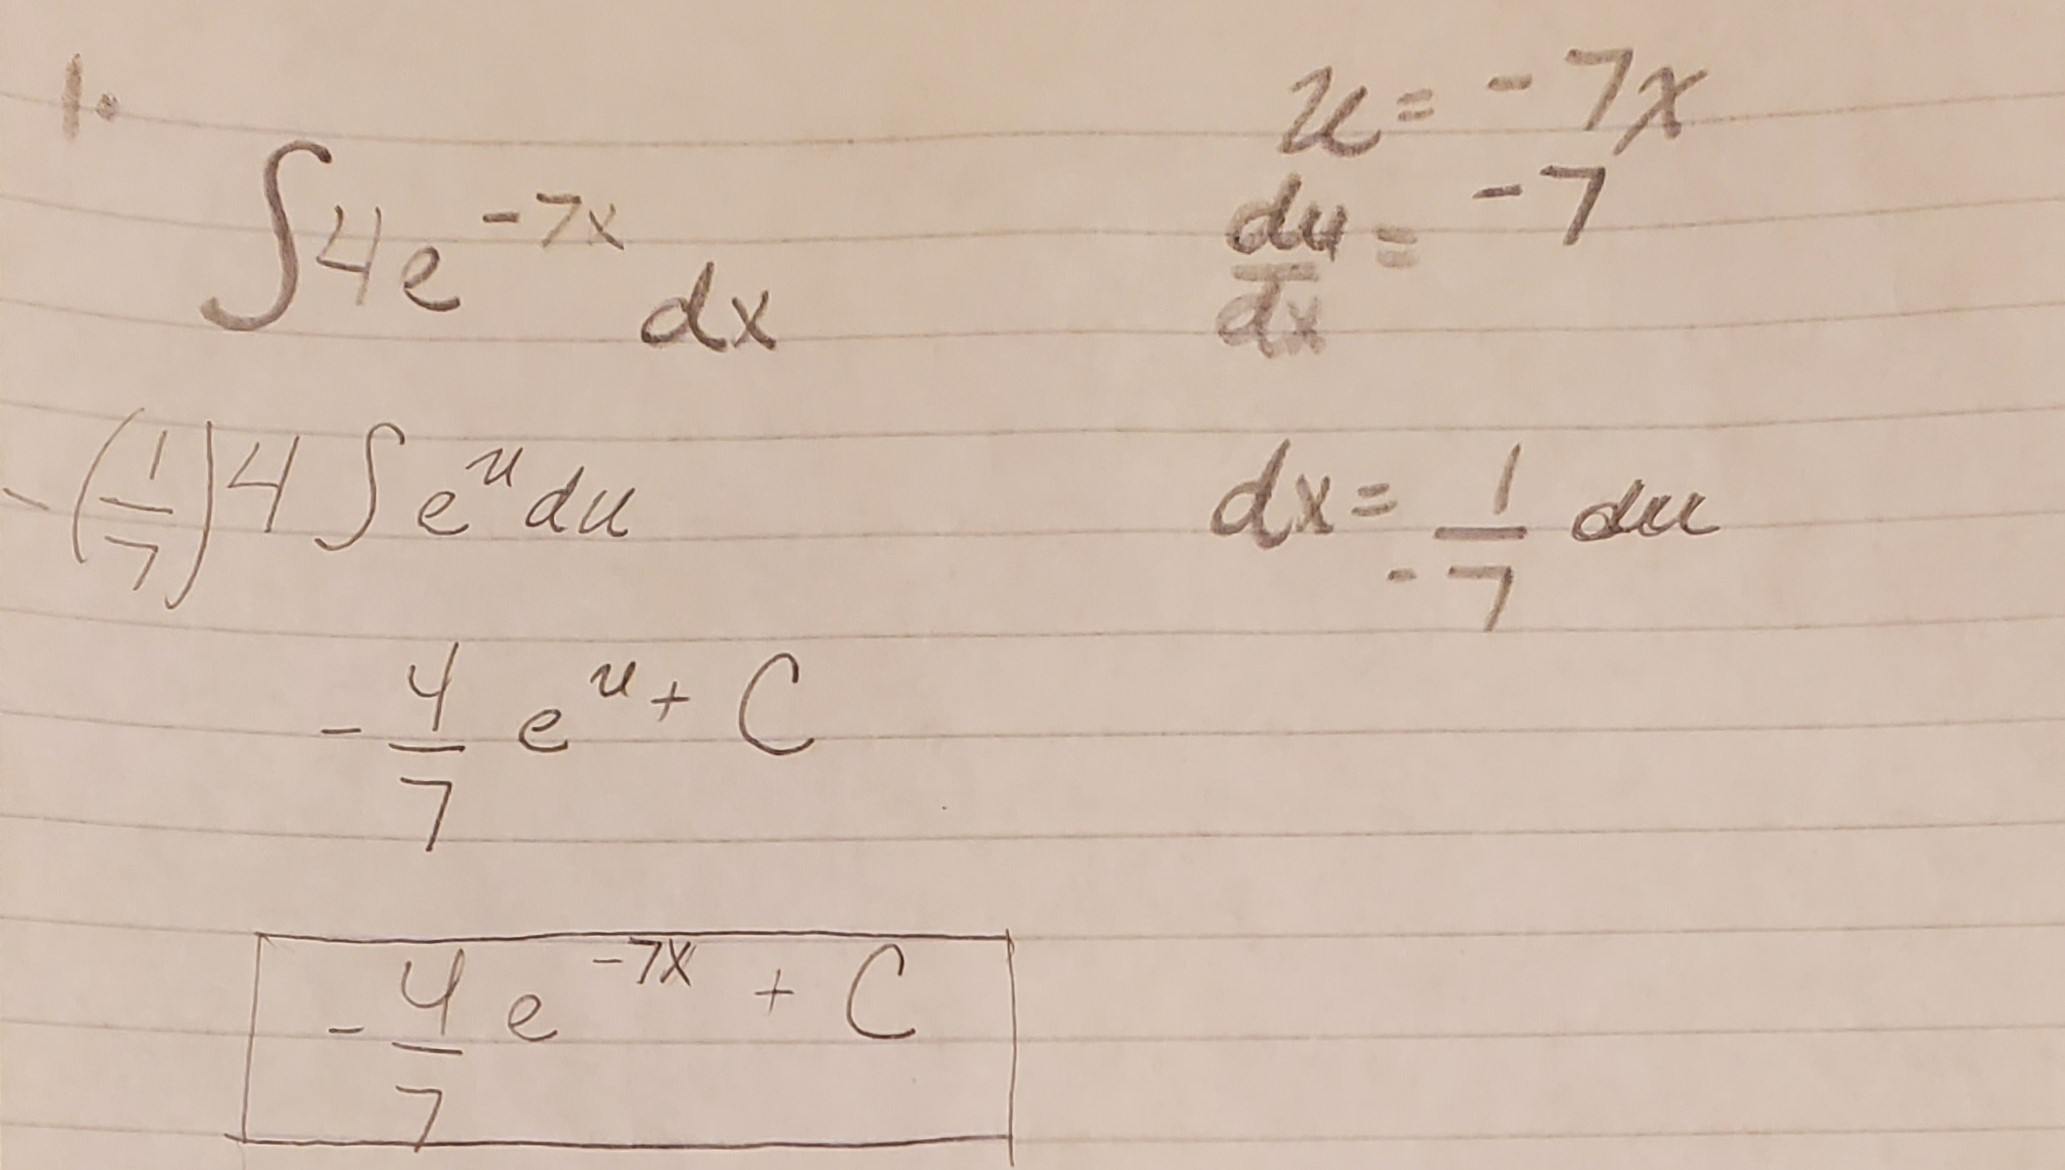
\includegraphics[width=28.68in]{13_1}

2.Biologists are treating a pond contaminated with bacteria. The level
of contamination is changing at a rate of dN dt =  3150 t 4  220
bacteria per cubic centimeter per day, where t is the number of days
since treatment began. Find a function N( t ) to estimate the level of
contamination if the level after 1 day was 6530 bacteria per cubic
centimeter.

\begin{Shaded}
\begin{Highlighting}[]
\NormalTok{knitr}\OperatorTok{::}\KeywordTok{include_graphics}\NormalTok{(}\StringTok{'13_2.jpg'}\NormalTok{)}
\end{Highlighting}
\end{Shaded}

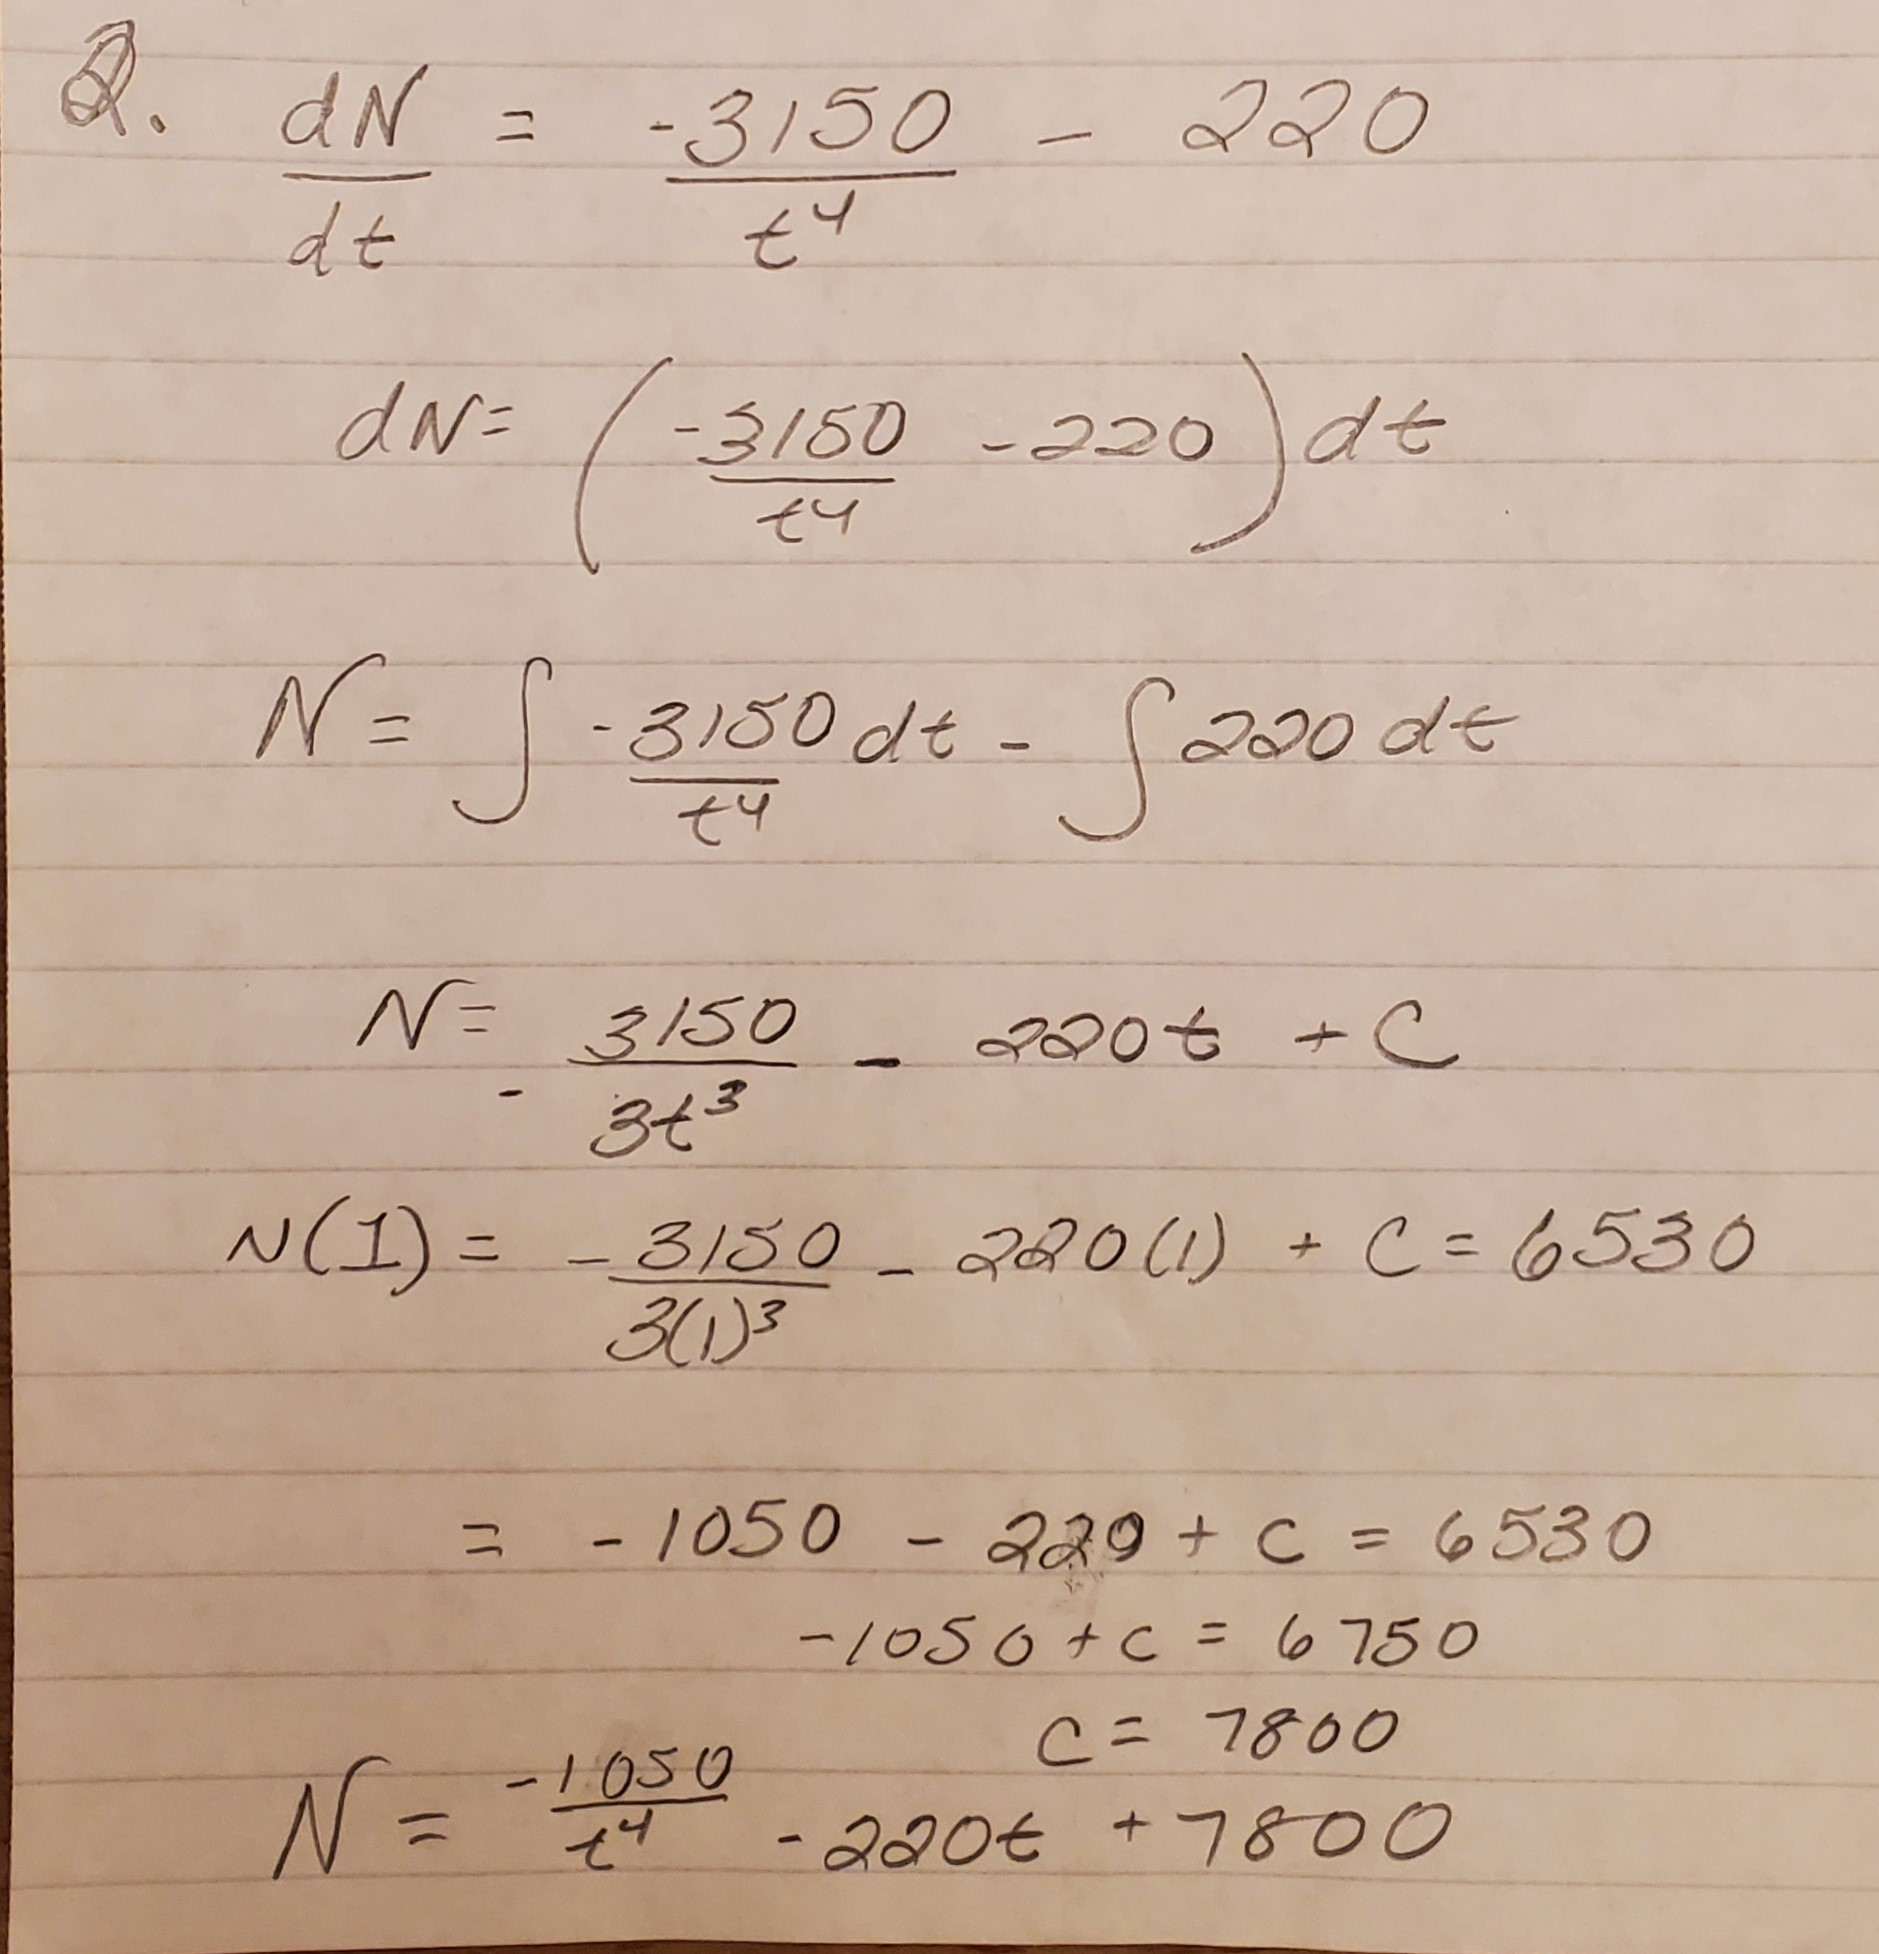
\includegraphics[width=26.1in]{13_2} 3.

Find the total area of the red rectangles in the figure below, where the
equation of the line is f ( x ) = 2x - 9.

\begin{Shaded}
\begin{Highlighting}[]
\NormalTok{prob_func<-}\StringTok{ }\ControlFlowTok{function}\NormalTok{(x)\{}
    \DecValTok{2}\OperatorTok{*}\NormalTok{x}\DecValTok{-9}
\NormalTok{\}}
\NormalTok{area <-}\StringTok{ }\KeywordTok{integrate}\NormalTok{(prob_func, }\DataTypeTok{lower =} \FloatTok{4.5}\NormalTok{, }\DataTypeTok{upper=}\FloatTok{8.5}\NormalTok{)}
\NormalTok{area}
\end{Highlighting}
\end{Shaded}

\begin{verbatim}
## 16 with absolute error < 1.8e-13
\end{verbatim}

\begin{enumerate}
\def\labelenumi{\arabic{enumi}.}
\setcounter{enumi}{3}
\tightlist
\item
  Find the area of the region bounded by the graphs of the given
  equations. y = x2 - 2x - 2, y = x + 2 Finding the zeroes:
\end{enumerate}

\begin{Shaded}
\begin{Highlighting}[]
\NormalTok{knitr}\OperatorTok{::}\KeywordTok{include_graphics}\NormalTok{(}\StringTok{'13_4.jpg'}\NormalTok{)}
\end{Highlighting}
\end{Shaded}

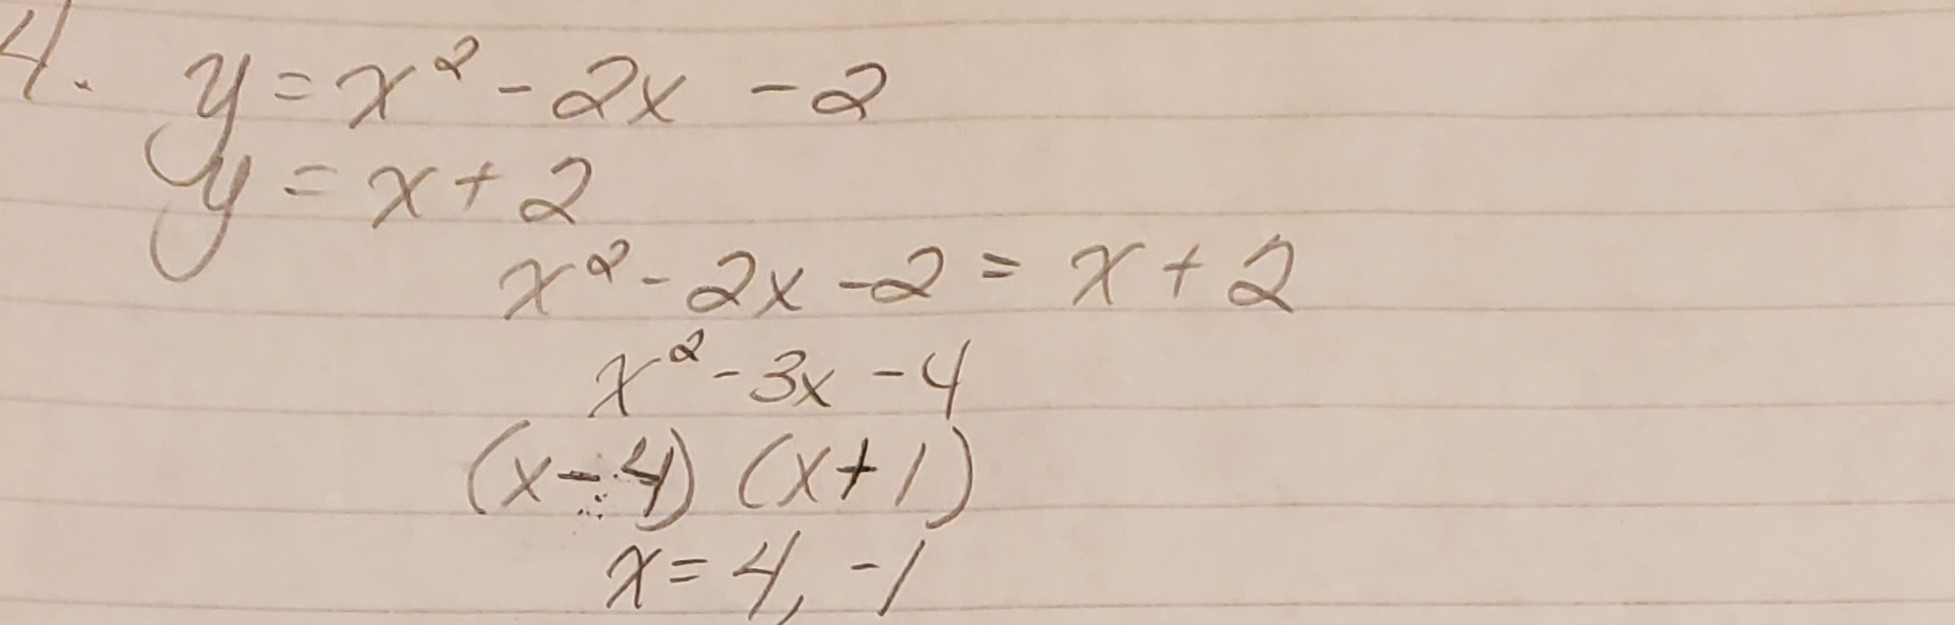
\includegraphics[width=27.15in]{13_4}

\begin{Shaded}
\begin{Highlighting}[]
\NormalTok{integrate_}\DecValTok{4}\NormalTok{ <-}\StringTok{ }\ControlFlowTok{function}\NormalTok{(x) \{ x }\OperatorTok{+}\StringTok{ }\DecValTok{2} \OperatorTok{-}\StringTok{ }\NormalTok{(x}\OperatorTok{**}\DecValTok{2} \OperatorTok{-}\StringTok{ }\DecValTok{2}\OperatorTok{*}\NormalTok{x }\OperatorTok{-}\StringTok{ }\DecValTok{2}\NormalTok{)\}}

\NormalTok{area <-}\StringTok{ }\KeywordTok{integrate}\NormalTok{(integrate_}\DecValTok{4}\NormalTok{, }\DecValTok{-1}\NormalTok{, }\DecValTok{4}\NormalTok{)}

\NormalTok{area}
\end{Highlighting}
\end{Shaded}

\begin{verbatim}
## 20.83333 with absolute error < 2.3e-13
\end{verbatim}

\begin{enumerate}
\def\labelenumi{\arabic{enumi}.}
\setcounter{enumi}{4}
\item
\end{enumerate}

A beauty supply store expects to sell 110 flat irons during the next
year. It costs \$3.75 to store one flat iron for one year. There is a
fixed cost of \$8.25 for each order. Find the lot size and the number of
orders per year that will minimize inventory costs.

\begin{Shaded}
\begin{Highlighting}[]
\NormalTok{knitr}\OperatorTok{::}\KeywordTok{include_graphics}\NormalTok{(}\StringTok{'13_5.jpg'}\NormalTok{)}
\end{Highlighting}
\end{Shaded}

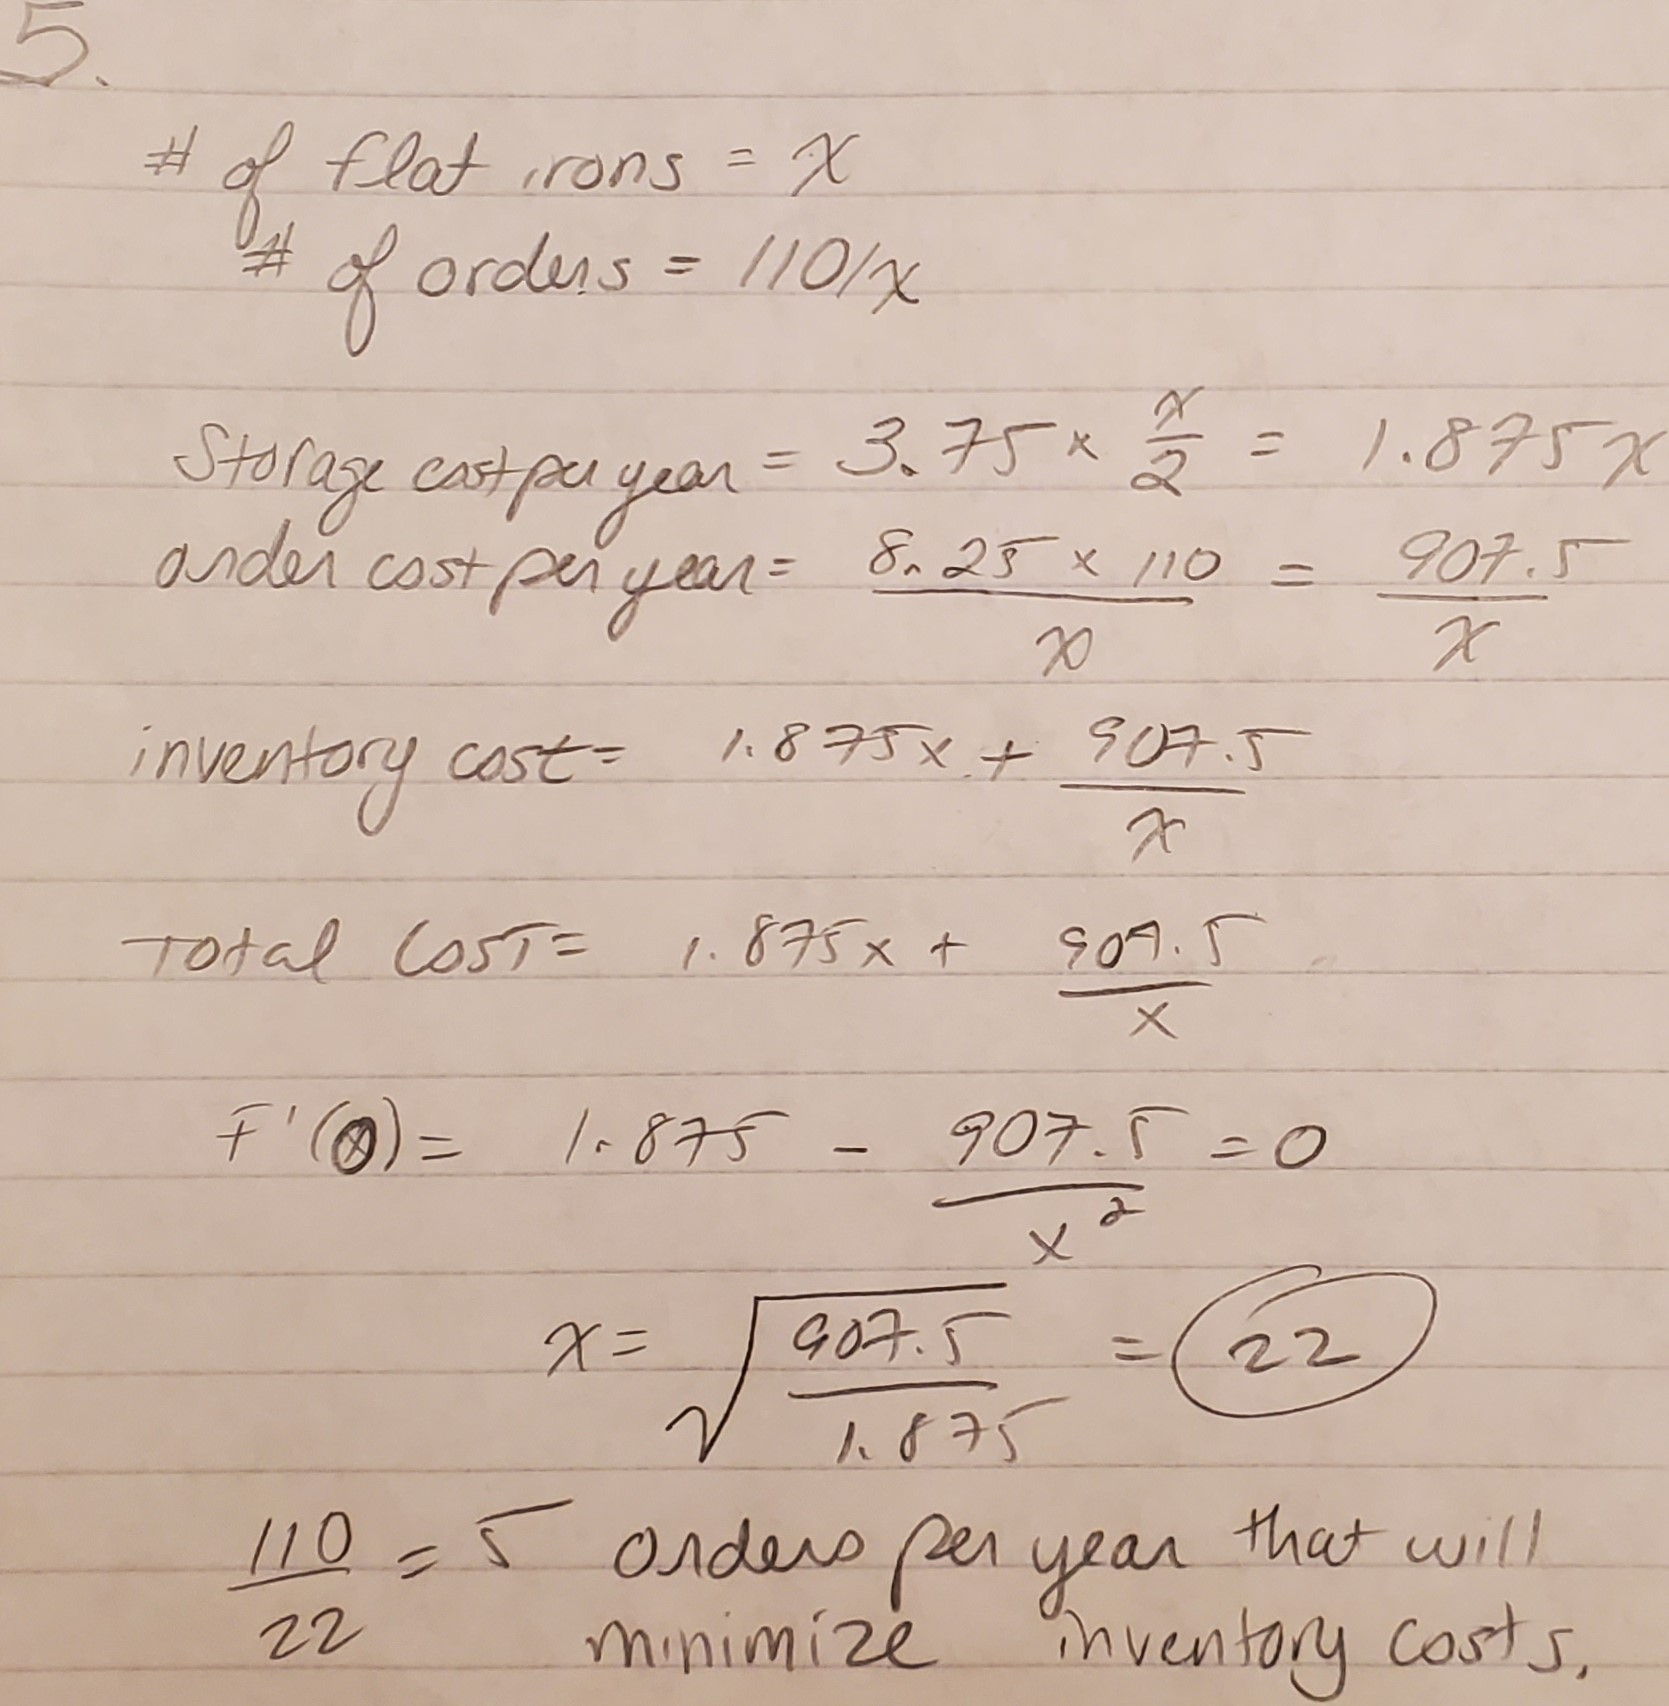
\includegraphics[width=23.18in]{13_5}

6.Use integration by parts to solve the integral below.

ln( 9x ) · x 6 dx

\begin{Shaded}
\begin{Highlighting}[]
\NormalTok{knitr}\OperatorTok{::}\KeywordTok{include_graphics}\NormalTok{(}\StringTok{'13_6.jpg'}\NormalTok{)}
\end{Highlighting}
\end{Shaded}

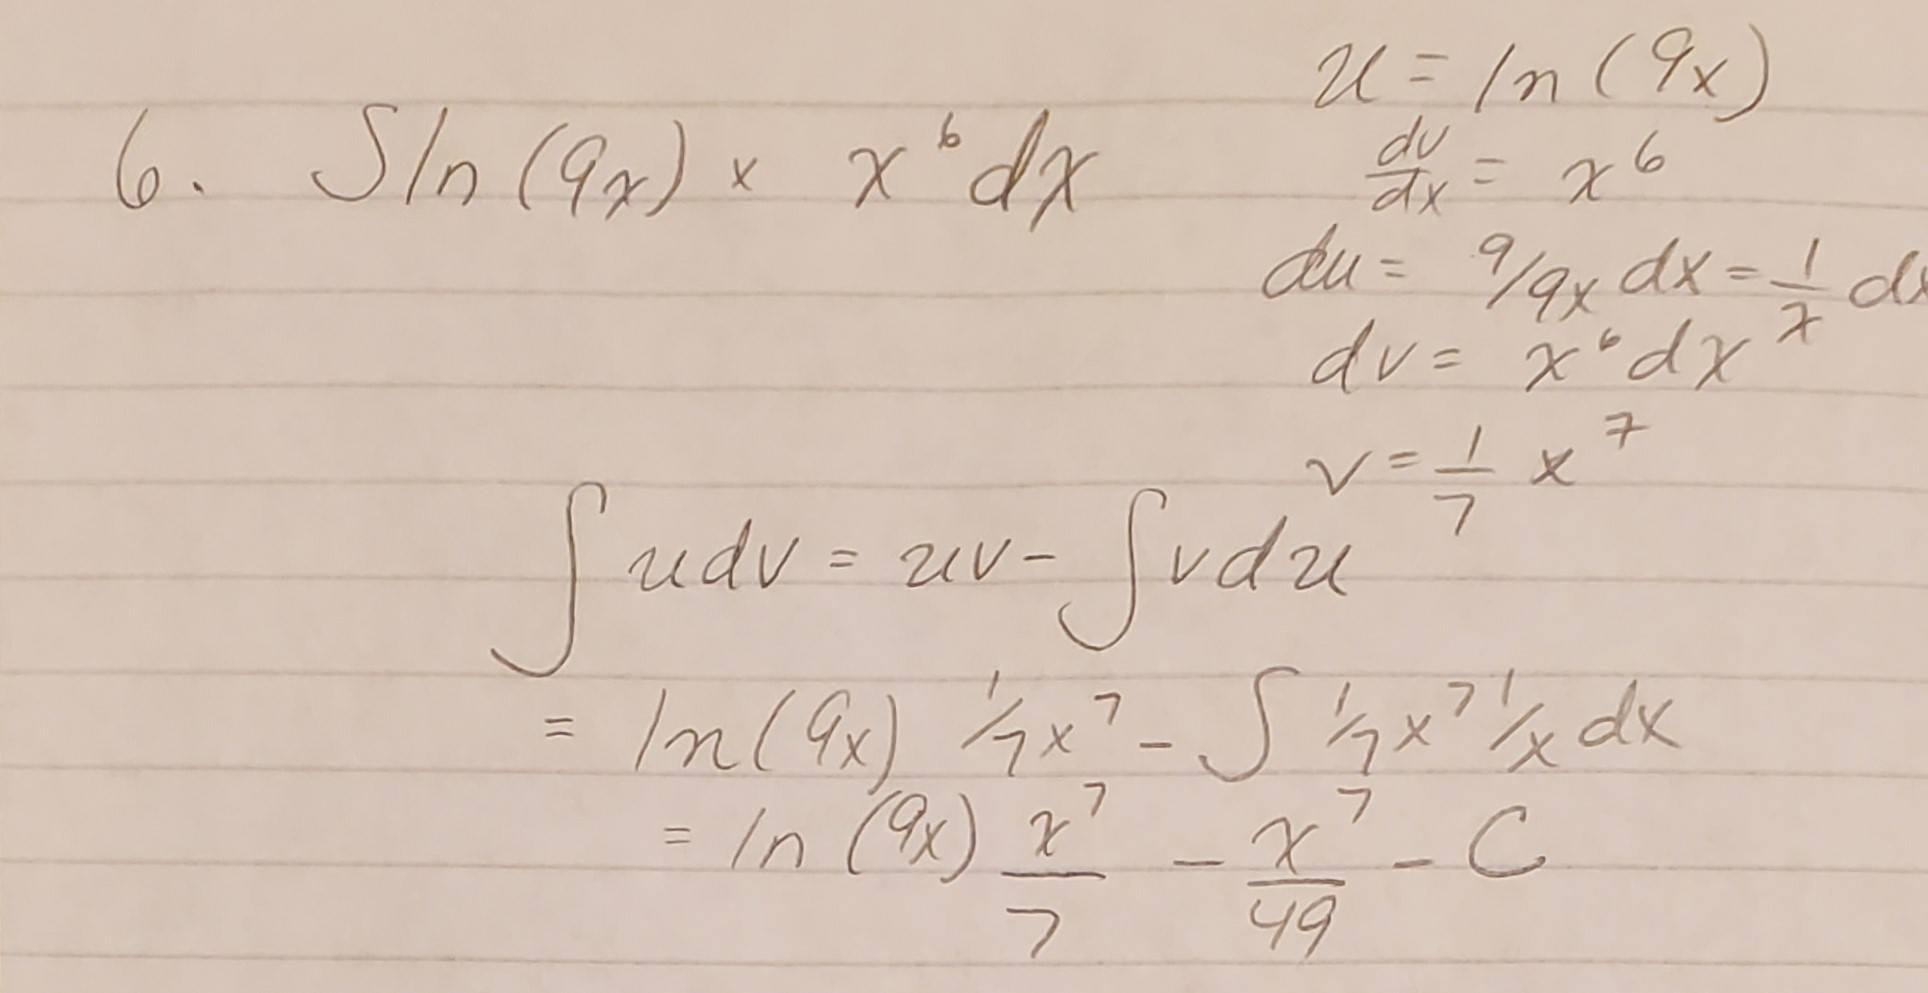
\includegraphics[width=26.78in]{13_6}

7.Determine whether f ( x ) is a probability density function on the
interval 1, e 6 . If not, determine the value of the definite integral.
f ( x ) = 1/6x

\begin{Shaded}
\begin{Highlighting}[]
\NormalTok{knitr}\OperatorTok{::}\KeywordTok{include_graphics}\NormalTok{(}\StringTok{'13_7.jpg'}\NormalTok{)}
\end{Highlighting}
\end{Shaded}

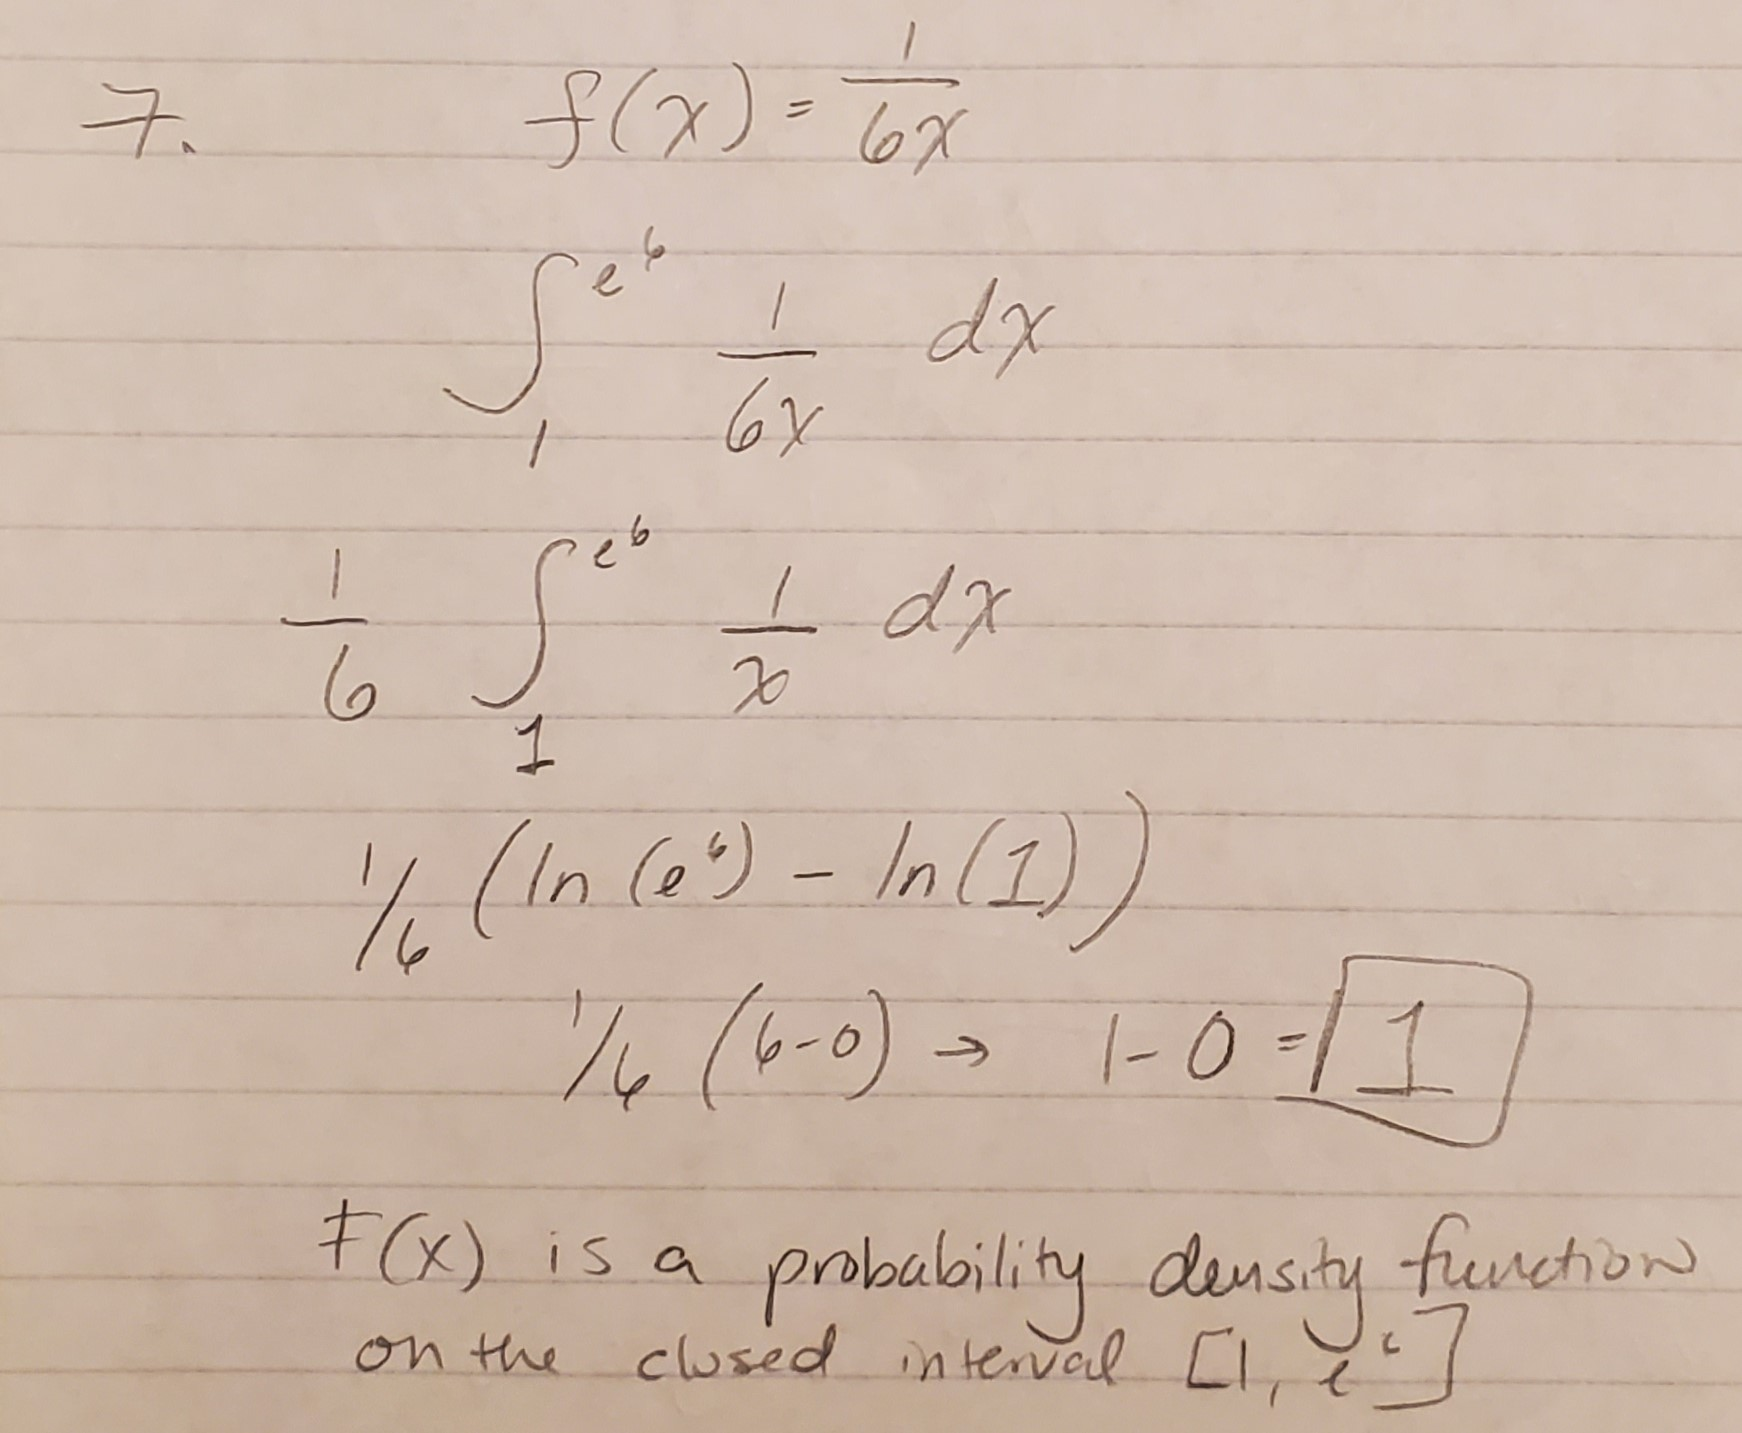
\includegraphics[width=24.19in]{13_7}

\end{document}
